% Please do not change the document class
\documentclass{scrartcl}

% Please do not change these packages
\usepackage[hidelinks]{hyperref}
\usepackage[none]{hyphenat}
\usepackage{setspace}
\usepackage{graphicx}
\graphicspath{ {G:/GitHubGames/comp110-architecture-essay/Pictures/} }
\usepackage[rightcaption]{sidecap}

\doublespace

% You may add additional packages here
\usepackage{amsmath}

% Please include a clear, concise, and descriptive title
\title{Implementation of PCG: Three Examples But Which Is The Easiest To Implement In A 2D Platformer?}

% Please do not change the subtitle
\subtitle{COMP110 - Computer Architecture Essay}

% Please put your student number in the author field
\author{1506530}

\begin{document}

\maketitle

\abstract{Procedural content generation (PCG) has been used in games for decades. It is an ever evolving method for creating immersive new content for the levels in games, that players can enjoy. This paper will describe three distinct algorithms for implementing PCG in a 2D platform game. Based on an analasis of relevant papers a recommendation will be made as to which algorithm would be the easiest to implement for a small indie company.}

\section{Introduction}

Procedural content generation (PCG) is one of many methods used today to create and design levels, particularity 2D platformers. PCG not only creates a new experience for the player with each play through, but also when done correctly can keep development costs down, by removing the need for extra level designers \cite{walaa}. The only real issue with PCG is which algorithm to choose, with the variety of algorithms that are available it can be daunting to decide on which direction to go. So with PCG its important to have a clear idea of the task you want to accomplish as this will clearly define which algorithm would be the best for that game. With this in mind this paper describes three different algorithms that could be used in a 2D Platform game. 
\newline
\newline
A brief description as possible for each algorithm and how they work are presented in the following sections. A comparison of ease of implementation into games will be drawn. Although looking at this, the recommended choice would be the ICA due to its simplicity and ease of use on more than one game. The three examples used are to be discussed on which algorithm would be the easiest to implement while still being the most efficient: An Iterative Content Adaptation Algorithm (ICA) used to enhance difficulty of a game \cite{fausto}; Genetic Algorithm (GA) used alongside an Agent-based Digger Algorithm to use and add assets to an established game \cite{walaa}; as well as an algorithm used alongside an input device to create a whole new game\cite{web}. More detailed information can be found in academic literature for example \cite{fausto,walaa,web}.
\newpage
\section{Iterative Content Algorithm (ICA)}

The first algorithm that is looked at is an ICA. It is considered interactive as it uses a graph overlay of a generated map to populate the map with objects and obstacles. Unlike other PCG levels where the level structure is produced from graphs, this algorithm requires each level to already be present to create something similar to the graph in Fig.1 Prince of Persia was used for these examples \cite{fausto}.


\begin{figure}[h!]
	\centering
	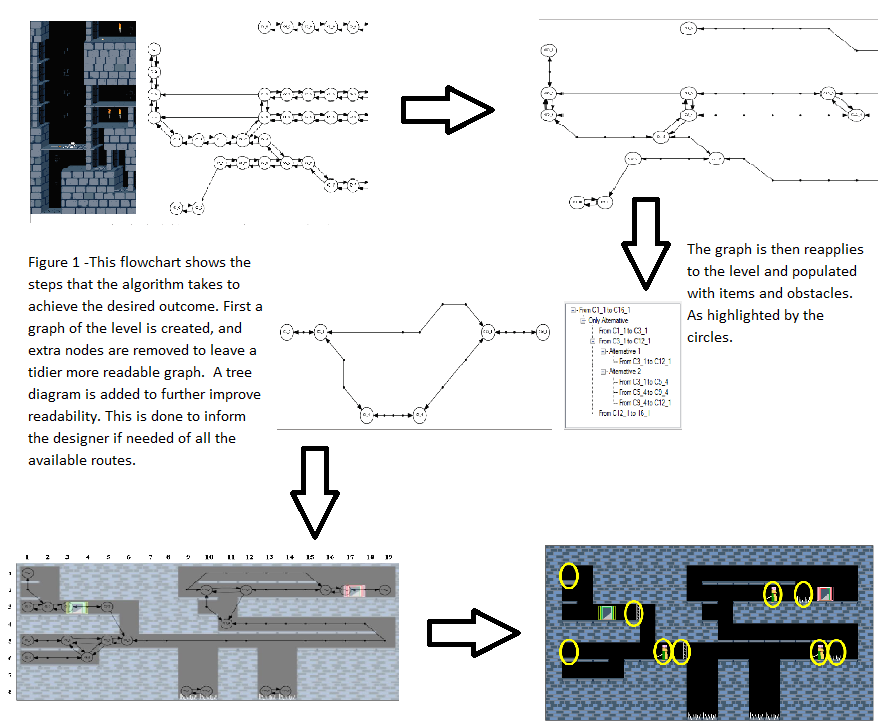
\includegraphics[width=1.0\linewidth]{Flowchart1}
	\caption{A summarised flowchart for the process of the ICA \cite{fausto}}
	\label{Fig1}
\end{figure}
\newpage
As can be seen from Fig.1 this particular method for PCG can be simple to implement. It does have limitations, one being that a level must already be created before implementation. Although it can also be put into multiple games with little to no modification see Fig.2,3. This makes it quite viable for a small indie company that can not afford the time to implement something with a greater complexity. Unlike the next method which takes it a step further by using a GA algorithm and created the entire level.


\begin{figure}[h]
	\centering
	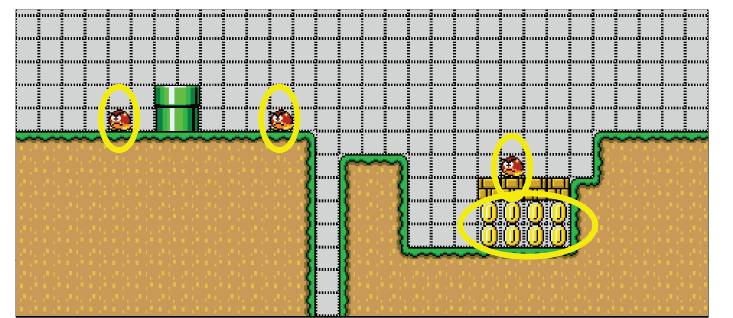
\includegraphics[width=0.9\linewidth]{Fig6}
	\caption{ - A Sample of a level from\textit{Infinite Mario Bros.} after the algorithm is applied \cite{fausto}}.
	\label{Fig2}
	\centering
	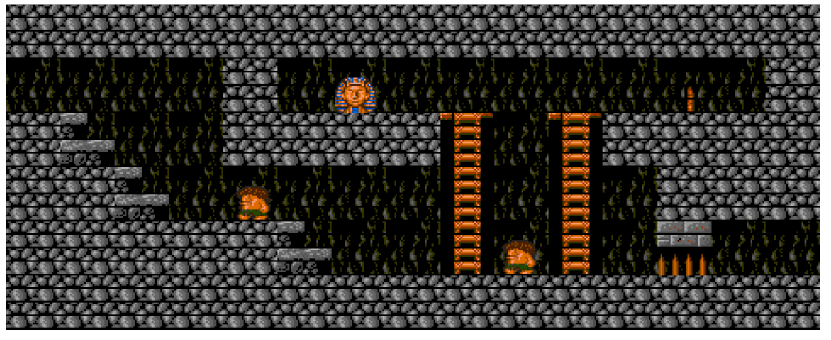
\includegraphics[width=0.9\linewidth]{Fig7}
	\caption{ - A Sample of a level from\textit{XRick} after the algorithm is applied \cite{fausto}}.
	\label{Fig3}
\end{figure}




\subsection{Genetic Algorithm (GA)}

Genetic Algorithm (GA) is a search heuristic that will mimic the natural selection process, a taxonomy of a evolutionary algorithm that runs through hundreds of evolutions to determine the most optimized method for the task at hand\cite{tax}. Infispel uses a Genetic Algorithm (GA) along with graphs of the rooms and the paths connecting them is used to populate the levels with items and objects Fig.4. \cite{walaa}.  

\begin{figure}[h!]
	\centering
	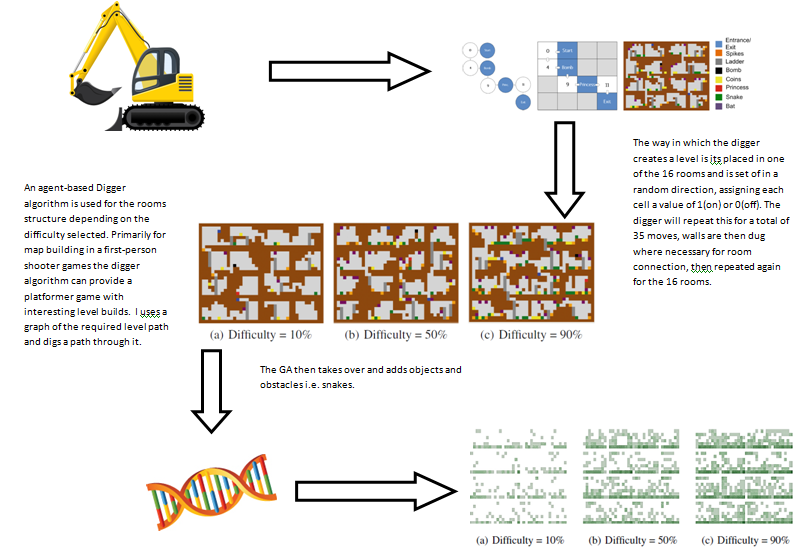
\includegraphics[width=1.0\linewidth]{Flowchart2}
	\caption{ - A summarised flowchart for the process of the GA and Digger algorithm\cite{walaa}}.
	\label{Fig4}
\end{figure}

Through this method a developer could create a PCG game based on these two Algorithms, but it would require modification before implementation unlike the ICA \cite{walaa,fausto}, but like the ICA this algorithm once implemented will create an interesting level based on the difficulty chosen.

\subsection{Endless Web (EW)}

The last and most complex method would be using the Launchpad along with a PCG algorithm to create a game that continuously builds the level depending on your play style\cite{web}. With EW, the approach taken was to use the Launchpads AI and as the controller followed by extensively modifying the mechanics to suit their needs.

\begin{figure}[h]
	\centering
	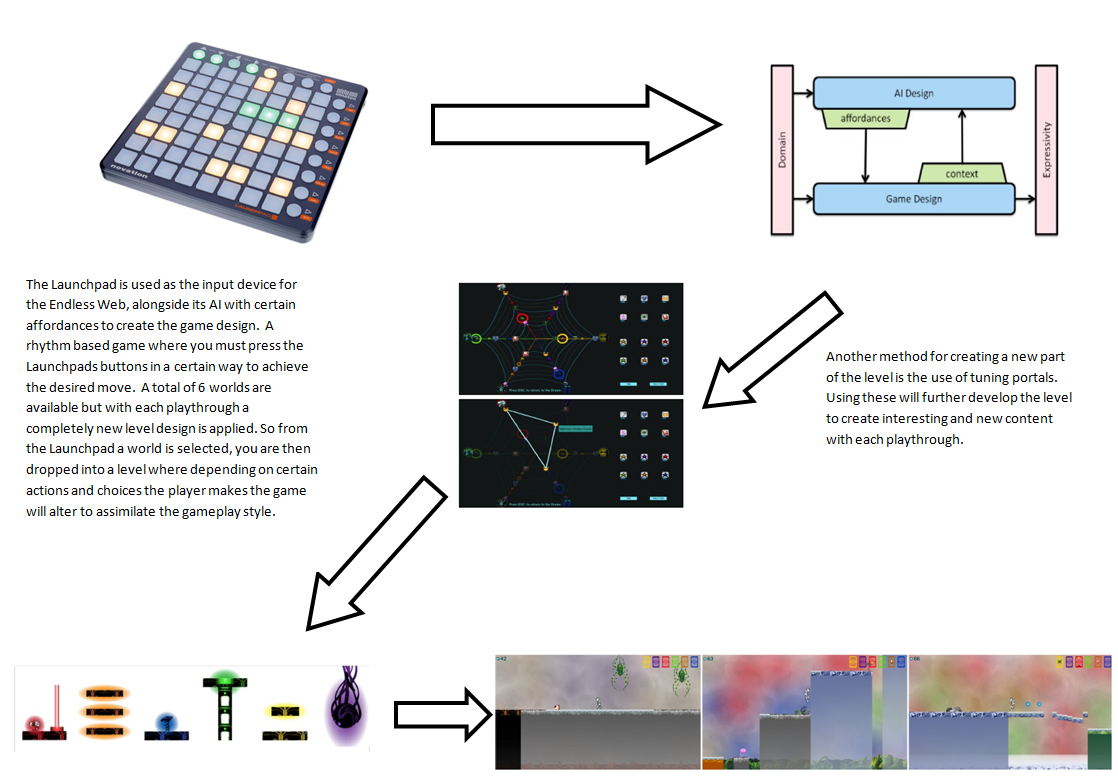
\includegraphics[width=1.0\linewidth]{Flowchart3}
	\caption{ - A summarised flowchart for the process of Endless Web\cite{web,web2}}.
	\label{Fig5}
\end{figure}

As can be derived from Fig.5 Endless Web has a greater complexity that the first two algorithms. This being said a game of this type can produce a far more personal experience\cite{web}. The development of such a PCG game would require a great deal of time and cost, for a small indie company it would be impractical to use such a method to create a game. For a company with more time and experience, this method would be a wise approach. 


\section{Conclusion}
As argued in section 2, the Iterative Content Algorithm (ICA) would be the most appropriate to use for a small 2D platform inide company. The ICA is the easiest most practical algorithm to implement into a PCG. It can support a wide variety of platform games with little to no modification \cite{fausto}. While the other two methods would require greater modifications and commitment to achieve\cite{walaa,web}
\newline
Although further research could be done with the three methods presented here, it is clear that PCG is still evolving in many directions. From small item placement as seen with the ICA to churning out an entire game as you play, as is seen in The Endless Web. From this paper it is hoped that the reader can take away a basic understanding of these three ways which PCG can be implemented into a 2D platform game. Along with a good idea of which method would be useful when creating a game for themselves. This paper is based on ease of implementation. A different metric could influence the recommendation offered.

\bibliographystyle{ieeetr}
\bibliography{comp110_architecture}

\end{document}
